\section{Ecosystem Simulator} \label{sec:ecosystem_simulator}

Once the user selects the union of all species that must appear in all clusters of the terrain, it is necessary to determine a valid vegetation distribution for each. To do so, an ecosystem simulator is used similarly to that in the work by Deussen et al \cite{Deussen1998} and Lane and Przemyslaw \cite{Lane2002}. Unlike these other ecosystem simulators, however, it isn't based on L-Systems and models both resource requirements and resource availability in greater detail. The purpose of ecosystem simulator is to determine, given a vegetative state, \textit{S$_{t}$} at time \textit{t}, the vegetative state \textit{S$_{t+n}$} at time \textit{t+n}, for any value of n. To do so, the simulation advances through time at monthly intervals and the strength of all plant instances are iteratively re-calculated. \\

\subsection{Gridded Simulation Area}

The simulation window greatly effects the performance of the ecosystem simulator and, therefore, it is necessary to keep it to a minimum. However, too small a simulation area will fail to accurately model the interaction of larger plant species. Given these constraints, a simulation window of \textbf{one hundred by one hundred meters} is used, accurate to the nearest centimetre. This area is deemed to be on the safe side, however, as rare are the species which come remotely close to such spatial coverage. An addition to this work would be to make the size of the simulation window vary depending on the  species selected to simulate. This would ensure optimal simulation speed for all simulation runs. \\

\begin{figure}
\center
	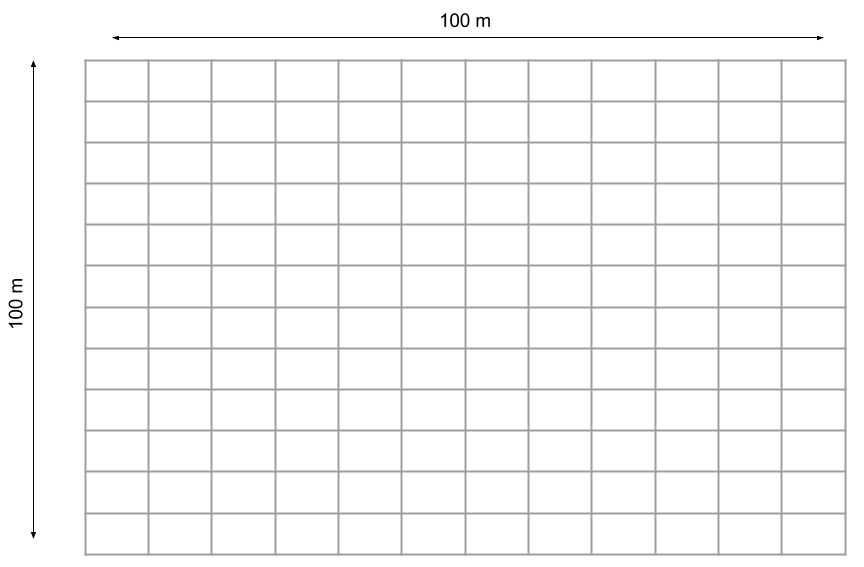
\includegraphics[width=\textwidth/2]{simulation_grid.png}
	\caption{ Gridded simulation area.}	
	\label{fig:simulation_grid}
\end{figure}

When iteratively calculating the strength of the plant instances present in the simulation, it is necessary to quickly determine the set of of plants S = \{P$_{1}$, P$_{2}$, P$_{3}$, ...\} with which they are competing for available resources. Determining \textit{S} depends on the spatial reach of \textit{P$_{n}$}. Spatial awareness is therefore a key requirement of the simulation and is achieved by splitting the simulation window into a grid of smaller cells as illustrated in figure \ref{fig:simulation_grid}.\\
The size of individual cells can be configured to increase/decrease the resolution and, therefore, the accuracy of the simulation. As the simulation progresses, plants grow, their spatial coverage increases, and they enter new grid cells. When a plant enters a new grid cell, it becomes a member of it and cell resources must be distributed to it. The information associated to each individual grid cell can be split into two categories: \textit{time-dependent} and \textit{simulation-dependent}. The time-dependent information depends only on the current month, is identical for every grid cell and is comprised of: the \textit{soil humidity} and the \textit{illumination}. The simulation-dependent information varies throughout the simulation as plants spawn, die and grow and is comprised of: the \textit{list of plants whose roots intersect the cell} and the \textit{list of plants whose canopy intersects the cell}.

\subsection{Humidity Distribution}

Plants grow there roots in order to access the nutrients and moisture available in the surrounding soil. As roots of different plant instances overlap, they start to compete for these resources. A notable simplification in our work is that soil depth is not modelled. Soil depth affects the plants rooting reach and has a significant impact on plant growth \cite{Fourcaud2008}. As an extension to this work, the soil could be modelled as layers which would permit plants to battle for different soil resources depending on their root coverage.\\

The strength of each plant in the simulation must be recalculated on a monthly basis. Part of the information required to calculate the overall strength of a given plant is the humidity allocated to it, which is taken as the average of the humidity allocated to it in each cell its roots overlap. To determine the overall humidity allocated to a given plant \textit{p}, it is first necessary, therefore, to iterate over all the grid cells and calculate the humidity allocated to each plant which roots are contained within.\\

When distributing the soil humidity of a given grid cell \textit{C$_{xy}$} to the set \textit{S} = \{P$_{1}$, P$_{2}$, P$_{3}$, ...\} of plants which roots intersect the cell, one of three distinct scenarios can occur, depending on the available humidity, \textit{H$_{available}$}, of the cell: \textit{Abundant humidity}, \textit{sufficient humidity} and \textit{insufficient humidity}.\\

The humidity is deemed abundant if the available humidity, \textit{H$_{available}$}, surpasses 300 millimetres. In this situation, the humidity is deemed to be enough for there to be standing water and therefore all plants of \textit{S} are allocated \textit{H$_{available}$}. \\

If \textit{H$_{available}$} is less than 300 millimetres, it is necessary to determine whether the humidity is sufficient or insufficient by calculating the requested humidity \textit{H$_{requested}$}, as outlined in equation \ref{eq:humidity_requested_calc}.

\begin{equation}
H_{requested} = \sum MinHumidity(P_{n}) \text{ for } n \in S
\label{eq:humidity_requested_calc}
\end{equation}
Where: \textit{MinHumidity(P$_{n}$)} is the minimum humidity requirement of the specie to which plant \textit{P$_{n}$} belongs; \textit{S} is the set of plants whose roots intersect with the given grid cell.\\

If \textit{H$_{requested}$} is less than \textit{H$_{available}$}, the humidity is deemed sufficient and the amount allocated to each plant is calculated as described in equation \ref{eq:humidity_allocation_sufficient_calc}.

\begin{equation}
\begin{split}
H_{allocated}(P_{n}) = MinHumidity(P_{n}) + OverFlow \\
OverFlow = H_{available} - \sum MinHumidity(P_{n}) \text{ for } n \in S
\end{split}
\label{eq:humidity_allocation_sufficient_calc}
\end{equation}
Where: \textit{H$_{allocated}$(P$_{n}$)} is the humidity allocated to plant \textit{P$_{n}$}; \textit{MinHumidity(P$_{n}$)} is the minimum humidity requirement of the specie to which plant \textit{P$_{n}$} belongs; \textit{S} is the set of plants whose roots intersect with the given grid cell.\\

If \textit{H$_{requested}$} is more than \textit{H$_{available}$}, however, the humidity is deemed insufficient and the allocation is done following equation \ref{eq:humidity_allocation_insufficient_calc}. Intuitively, this equation allocates each plant with the minimum amount of humidity it requires to survive plus the resulting overflow. It also prioritises water distribution to the more vigorous plants to ensure stronger plants have a greater chance of survival than weaker ones.

\begin{equation}
\begin{split}
H_{allocated}(P_{n}) = min(MinHumidity(P_{n}), Vigor(P_{n}) \times H_{remaining}) \\
Vigour(P_{n}) =  \frac{RootSize(P_{n})}{\sum RootSize(P_{x}) \text{ for } x \in S}\\
H_{remaining} = H_{available} - (\sum H_{allocated}(P_{x})  \text{ for } x \in S_{processed})\\
\end{split}
\label{eq:humidity_allocation_insufficient_calc}
\end{equation}
Where: The plants of \textit{S} \textbf{must} be iterated over in decrementing order of their vigor as this will affect the water allocated to them; \textit{H$_{allocated}$(P$_{n}$)} is the humidity allocated to plant \textit{P$_{n}$}; \textit{MinHumidity(P$_{n}$)} is the minimum humidity requirement of the specie to which plant \textit{P$_{n}$} belongs; \textit{Vigour(P$_{n}$)} is the vigour of plant \textit{P$_{n}$} in comparison to other plants present in the cell. It is estimated based on root size; \textit{RootSize(P$_{n}$)} is the root size of plant \textit{P$_{n}$}; S$_{processed}$) is the set of plants from \textit{S} whose water allocation has already been calculated; \textit{S} is the set of plants whose roots intersect with the given grid cell.\\

The overall allocated humidity to \textit{P$_{n}$} is calculated using equation \ref{eq:plant_humidity_allocation}. Intuitively, it is simply the average of all humidity allocated to it within all cells of \textit{S}.

\begin{equation}
H_{n} = \frac{\sum H_{allocated}(C_{x}) \text{ for } x \in S}{| S |}
\label{eq:plant_humidity_allocation}
\end{equation}
Where:\textit{H$_{n}$} is the humidity allocated to plant \textit{P$_{n}$}; \textit{S} = \{C$_{1}$, C$_{2}$, C$_{3}$, ...\} is the set of cells that the roots of plant \textit{P$_{n}$} intersect; \textit{H$_{allocated}$(C$_{n}$)} is the humidity allocated to plant \textit{P$_{n}$} in grid cell C$_{n}$; \textit{$|$ S $|$} is the number of cells in the set \textit{S}.

\subsection{Illumination Distribution}

Photosynthesis is an essential part of plant development which permits the creation of fresh matter and, therefore, growth \cite{Soler2001}. Species which are heavily dependent on illumination will often grow large canopies to maximize the leaf coverage area and therefore photosynthesis potential. These large canopies also limit the illumination available in the area underneath the canopy, limiting plant development. To model this, available illumination is calculated for each grid cell based on the height of the plants which canopy intersect the given cell as outline in equation \ref{eq:illum_distribution}. Intuitively, if all plants present in the given cell are canopy-free (i.e no shade projection), the equation allocates them all the available illumination. If not all plants are canopy-free, the equation allocates illumination only to the tallest canopy plant. Note that this is a simplification as some light should still pass through the canopy and the shade projected by the canopy is not always directly below but varies throughout the day and the year. A much more detailed approach is taken by Soler et al. \cite{Soler2001} who model light transmittance through the canopy based on plant geometry. This detailed approach is ill-suited here, however, as the growth of a large set of plants needs to be simulated simultaneously. A possible extension to this work would be to associate with each plant species a canopy density parameter which affects the quantity of light which can pass through its canopy.

\begin{equation}
\centering
Illumination(C_{xy}, P_{n}) = 
\begin{cases}
	C_{illumination}, & \text{if } CanopyWidth(P) = 0 for P \in S \\
	C_{illumination}, & \text{if } Height(P_{n}) > height(P) for P \in S : P \neq P_{n} \\
    0,              & \text{otherwise}
\end{cases}
\label{eq:illum_distribution}
\end{equation}
Where: \textit{Illumination($P_{n}$)} is the illumination allocated to plant \textit{P$_{n}$} whose canopy overlaps grid cell C$_{xy}$; \textit{C$_{illumination}$} is the available illumination for the given month (equal for all cells);\textit{CanopyWidth(P)} is the canopy width of plant \textit{P}; \textit{Height(P)} is the height of plant \textit{P}; \textit{S} is the set of plants whose canopy intersects with the given grid cell \textit{C$_{xy}$}.\\

Calculating the illumination allocated to a plant \textit{P$_{n}$} is identical to calculating the humidity allocated (see equation \ref{eq:plant_humidity_allocation}) but the cells considered are those which the plants canopy intersects (and not its roots). Intuitively, the illumination allocated to a given plant is simply the average of the humidity allocated to it in all grid cells its canopy intersect.

\subsection{Plant Strength Calculation} \label{subsec:plant_strength_calc}

Given the humidity and illumination allocated to a given plant \textit{P}, the temperature, the slope and the age of \textit{P}, it is possible to calculate its overall strength, which is subsequently used as a representation of the plants health and directly affects its growth and survival. \\
The overall strength, of plant \textit{P}, is taken as the minimum of \textit{S$_{slope}$}, \textit{S$_{age}$}, \textit{S$_{temperature}$}, \textit{S$_{illumination}$} and \textit{S$_{humidity}$} which represent the strength of \textit{P} in terms of the slope, its age, the temperature, the allocated illumination and humidity, respectively. The minimum is taken rather than the average as the strength of a plant should depend heavily on the limiting resource. For example, if a plant is struggling to due a lack of daily illumination, improving the allocated water should not have a big impact on its overall health.\\
To calculate the individual strength values, which range from negative to positive one hundred, a graph is plotted as outlined in figures \ref{fig:2_value_strength} and \ref{fig:4_value_strength} for each species based on its associated properties (see section \ref{sec:plant_species}). Using these, it is possible to calculate the plants strength in terms of slope, age, temperature, illumination and humidity.

\begin{figure}
\center
	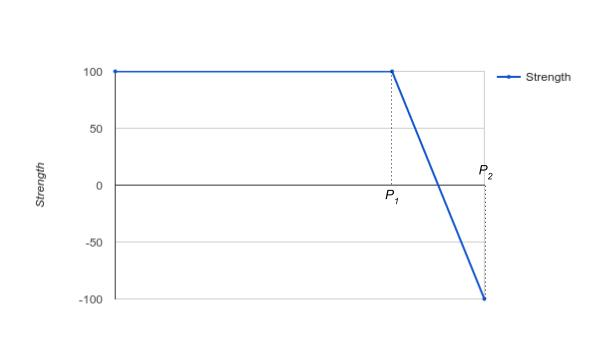
\includegraphics[scale=0.7]{2_value_strength.jpg}
	\caption{ Graph used to calculate the slope and age strength of a given plant instance where: \textbf{P$_{1}$} represents the value of \textit{start of decline} and \textbf{P$_{2}$} is the \textit{maximum} configured for the given specie. }	
	\label{fig:2_value_strength}
\end{figure}

\begin{figure}
\center
	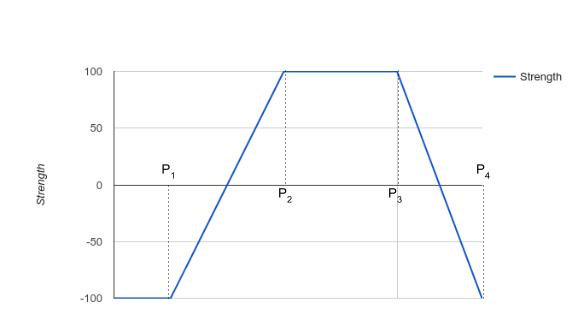
\includegraphics[scale=0.7]{4_value_strength.jpg}
	\caption{ Graph used to calculate the temperature, illumination and humidity strength of a given plant instance where: \textbf{P$_{1}$} and \textbf{P$_{4}$} are the \textit{minimum} and \textit{maximum} and \textbf{P$_{2}$} and \textbf{P$_{3}$} form the \textit{prime range} configured for the given specie.  }	
	\label{fig:strength_calc_temp}
\end{figure}

\subsection{Plant Growth}

In the simulation, each plant \textit{P} attempts to grow its roots, its canopy and it's height on a monthly basis. Each specie has an maximum monthly root growth, canopy growth and height growth which are calculated as outlined in equation \ref{eq:max_growth}. It uses the maximum height, canopy and root size along with the species age of start of decline (see section \ref{sec:plant_species}) to calculate the amount it must grow each month to reach these maximums by the time it reaches the age of start of decline. Note that this is a simplification as, in reality, plant growth is non-linear as growth slows with increasing size \cite{Paine2012}.

\begin{equation}
MaxGrowth(S) = \frac{Max(S)}{Age_{sod}(S)}
\label{eq:max_growth}
\end{equation}
Where:\textit{MaxGrowth(S)} is the maximum monthly root, canopy or height growth of specie \textit{S}; \textit{Max(S)} is the maximum root size, canopy size or height configured for specie \textit{S}; \textit{Age$_{sod}$(S)} is the age of start of decline configured for specie \textit{S}.\\

The actual root growth, canopy growth and height growth is directly dependent on its strength (see section \ref{subsec:plant_strength_calc}), however, and is calculated using equation \ref{eq:actual_growth}. This equation only permits growth if the plant's strength is positive as the plant is otherwise considered in a \textit{survival state}. If the strength is positive, the growth is proportional to the plants strength. The maximum growth is therefore only achieved if the plant is at its full strength.\\

\begin{equation}
Growth(\textit{P},S) = max(0, Strength(\textit{P}) \times  MaxGrowth(S)
\label{eq:actual_growth}
\end{equation}
Where: \textit{Growth(S)} is the monthly root, canopy or height growth of plant \textit{P} of specie \textit{S}; \textit{Strength(\textit{P}} is the current strength of \textit{P}; \textit{MaxGrowth(S)} is the maximum monthly root, canopy or height growth calculated for specie \textit{S} (see equation \ref{eq:max_growth}).

\subsection{Plant Death}

In order for the simulation to be accurate, it is necessary to model plant death. This can be caused by its age, the slope being ill-suited or resources being inadequate. On a monthly basis, the probability of death of each plant is calculated based on its strength using equation \ref{eq:probability_of_death} and the plant killed off with the given probability. This equation permits plants to be killed-off when in a survival state (i.e the strength is negative). If this is the case, the probability of death is proportional to the absolute value of strength. 

\begin{equation}
Probability_{death}(P) = max(0, \frac{-1 \times Strength(P) + counter}{100})
\label{eq:probability_of_death}
\end{equation}
Where:\textit{Probability{death}(P)} is the probability of death of plant \textit{P};\textit{Strength(\textit{P}} is the current strength of \textit{P};\textit{counter} is a value which increases each month the plant's strength is negative and resets to zero when it becomes positive. This is to prevent plants from surviving in a survival state for too long.

\subsection{Spawning Plants} \label{subsec:spawning_plants}

In nature, the spawning of new plants ensures species \textit{succession} and \textit{propagation}. In order to accurately model the evolution of an ecosystem it is essential to replicate this spawning mechanism. To do so, seeds are produced annually for each specie and are positioned either randomly or at predefined positions. The number of seeds that are produced for a given specie is determined by the species configured \textit{annual seed count}. Different seeding mechanisms are used in the simulator depending on the current state of the simulation, as discussed below.\\ 

To ensure specie propagation, when plant's of the given specie are already present in the simulation window, they are used to determine the location for new plant instances. To do so, \textit{n} of these plants are selected at random and seeds placed at random within an annular radius \textit{r} of each. The value of \textit{n} is the \textit{annual seed count} configured for the current specie. The value of \textit{r} is the configured \textit{maximum seeding distance} of the specie. Note that a single plant can be used to spawn multiple seeds if \textit{n} is greater than the number of plants of the given species present in the simulation.\\
This technique is effective in ensuring \textit{propagation} until the number of plant instances present far outweighs the number of seeds to produce, at which point, the \textit{propagation} potential decreases. This is because, as the selection pool for the random seeding plants increases in size, the probability of selecting a plant at a location which will permit propagation decreases. To overcome this and ensure the initial seeding plants that are selected span a wide area, the simulation window is split into equally sized cells and the seeding plants selected individually from each. \\

If no instance of the given specie is present in the simulation (i.e it is the first month) and therefore no seeding plants can be used, the seeds are placed at random within the simulation window.\\ 

A specie is deemed shade-loving if its configured minimum daily illumination is zero. Such species strive in the undergrowth of other plants. Spawning shade-loving species in the same way as other plants would drastically limit there chance of survival. The reason for this is that the probability of the randomly selected seed location to be the canopy of an existing plant is very low. For this reason, when there are no instances of the given shade-loving specie present in the simulation window, the seed locations are now selected at complete random but at random under the canopy of existing plants. If instances of the plant specie are already present, however, they are used to propagate the seeds, just like with other, non shade-loving, plant species.

\subsection{Performance} \label{subsec:ecosytem_performance}

The number of plants present in the simulation will heavily influence it's performance as the strength of each plant needs to be recalculated on a monthly basis. To test the influence of plant count on simulation time, a simulation is run with a single specie of plant and the monthly processing time analysed alongside the number of plants present. The plant used is grass as is has no canopy and very minimal root coverage, therefore permitting a large number of instances to grow simultaneously (see appendix \ref{AppendixB} for properties of the specie). The resources were set to be optimal for maximizing plant count and minimizing intra-plant competition. The simulation is started with only a single instance and, as the simulation progresses and seeding is performed, the number of instances increases. The results are summarized in Figure \ref{fig:ecosimulator_test_plant_count} and show that the processing time increases linearly with plant count. \\

\begin{figure}
\center
	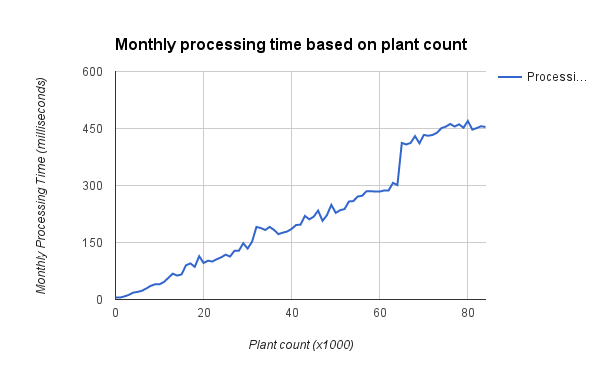
\includegraphics[scale=0.7]{ecosimulator_test_plant_count.png}
	\caption{ Processing time based on plant count. Total simulation time for 100 years: 271 seconds}	
	\label{fig:ecosimulator_test_plant_count}
\end{figure}

Another property which heavily impacts performance is the root and canopy growth of plant species present. The reason for this is that, as plants roots and canopy grow, they will cover more grid cells of the simulation window. As a consequence, more calculations will be required per individual cell when the resources are distributed within. To analyse the impact of plant growth, a base specie \textit{S$_{base}$} is created with a given root and canopy growth rate. Then, two species \textit{S$_{X2}$} and \textit{S$_{X3}$} are created with identical properties to \textit{S$_{base}$} but with twice and thrice the growth rates, respectively (see appendix \ref{AppendixB} for specie details). An separate identical simulation is run with each specie in terms of available resources and, on a monthly basis, the number of plants present in the simulation, along with the monthly processing time, analysed. Given this information, it is possible to track the average monthly processing time per plant throughout the simulation. It is important to normalise based on the number of plants as faster growing plants will naturally reduce the total plant count for the simple reason that they will require and be able to access resources from a larger amount of grid cells. As can be seen in the results plotted in figure \ref{fig:ecosimulator_test_per_plant}, the processing times are similar to start and then increase proportionally to the species growth rate. For the fastest growing plant specie, \textit{S$_{X3}$}, it took 166 seconds to simulate one hundred years.

\begin{figure}
\center
	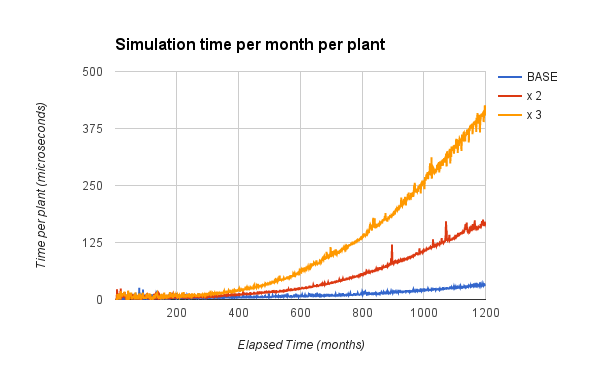
\includegraphics[scale=0.7]{ecosimulator_test_per_plant.png}
	\caption{ Evolution of the monthly processing time normalised based on plant count. The processing time increases as the plant's grow larger as they cover more grid cells. Total simulation time for one hundred years: ~49 seconds for \textit{S$_{base}$}, ~122 seconds for \textit{S$_{X2}$} and 166 seconds for \textit{S$_{X3}$}}
	\label{fig:ecosimulator_test_per_plant}
\end{figure}

\subsection{Results}

To test the resulting spatial distribution of plant communities in their work, Lane and and Przemyslaw \cite{Lane2002} attempt to reproduce three important properties of nature: \textit{Self-thinning}, \textit{succession} and \textit{propagation}. To test the ecosystem simulator, we employ the same methodology as Lane and and Przemyslaw \cite{Lane2002} and attempt to reproduce these core properties of nature. Other tests are also performed to ensure plant instances thrive better in environments better suited to their resource requirements.\\

\textbf{SELF-THINNING TEST}\\

As plants grow, their resource requirements increase and, as a direct consequence, inter-plant competition for resources increases. Eventually, the competition becomes too intense and resources too scarce leading to more vigorous plants starving smaller plants. At this point, \textit{self-thinning} begins and plant densities decrease.\\
To test whether self-thinning is successfully modelled in the ecosystem simulator, three simulations are run as described in table \ref{tab:self_thinning_test_simulations} and the plant count tracked throughout. As described previously, self-thinning occurs because of insufficient resources. By modifying only available humidity in each simulation, its affect on self-thinning becomes apparent. As can be seen in the results summarized in figure \ref{fig:self_thinning_test_results}, the plant count increases at first, reaches a maximum and decreases thereafter. This is the exact behaviour of self-thinning. Furthermore, it is apparent that the maximum plant count increases with the humidity available, therefore showing that the tipping point depends on available resources.\\

\begin{table}[]
  \centering
	    \begin{tabular}{|p{2cm}|p{2cm}|p{2cm}|p{2cm}|p{2cm}|p{2cm}|}
		\hline
		\textbf{Simulation} & \textbf{Simulation time (years)} & \textbf{Humidity} & \textbf{Illumination} & \textbf{Temperature} & \textbf{Slope}\\
		\hline       
		1 & 100 & 25 & 10 & 15 & 0\\           
		\hline       
		2 & 100 & 30 & 10 & 15 & 0\\   
		\hline       
		3 & 100 & 35 & 10 & 15 & 0\\              
		\hline       
		\end{tabular}
		\caption{Self-thinning test simulation configurations. For simplicity, monthly resources are kept constant.}
		\label{tab:self_thinning_test_simulations}
\end{table}

\begin{figure}
\center
	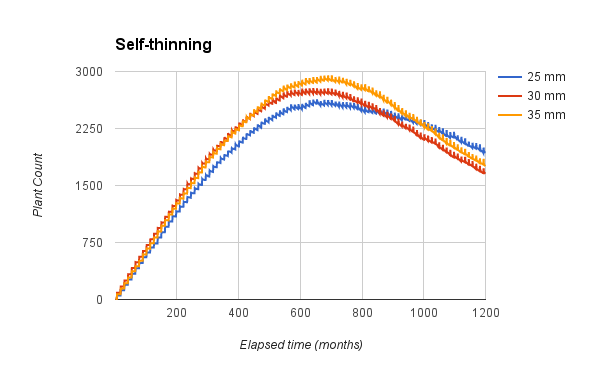
\includegraphics[scale=0.7]{self_thinning.png}
	\caption{ Self thinning test: plant count tracked throughout three separate simulations differing only in available humidity. For all three runs the plant density reaches a maximum tipping-point after which plant density reduces.}
	\label{fig:self_thinning_test_results}
\end{figure}

\textbf{SUCCESSION TEST}\\

Given plant specie \textit{A} with a fast growth rate and specie \textit{B} with a slower growth rate but higher shade tolerance. At first, the faster growing specie A will dominate and flourish but, with time, the slower growing, but more shade-tolerant specie B will flourish and dominate. This is the \textit{succession} property. To test \textit{succession} in the ecosystem simulator, two plant species \textit{S$_{fast}$} and \textit{S$_{slow}$} are created differing only in their growth rate and illumination properties (see appendix \ref{AppendixB} for details) and a simulation run with these two species under optimal conditions. During the simulation, the appearance and average size of the two plant species are monitored to determine the dominating specie. The results are analysed and illustrated in figure \ref{fig:succession_plants_avg_size}. A snapshot of the simulation window is taken at ten year intervals and displayed in figure \ref{fig:succession_plants_render}. Both these figures show that \textit{S$_{fast}$} dominates at first (~300 months in) followed by \textit{S$_{slow}$} (~500 months in). A balance is found thereafter.\\

\begin{figure}
\center
	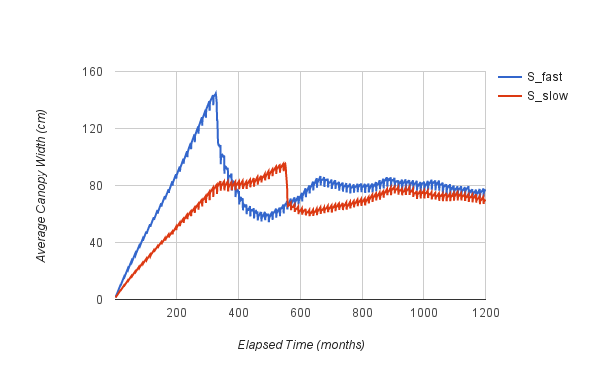
\includegraphics[scale=0.7]{succession_plant_avg_size.png}
	\caption{ Succession Test: Average size of the slow growing S$_{slow}$ (red) and fast growing S$_{fast}$ (blue) throughout a simulation run in optimal conditions. }
	\label{fig:succession_plants_avg_size}
\end{figure}

\begin{figure}
\center
	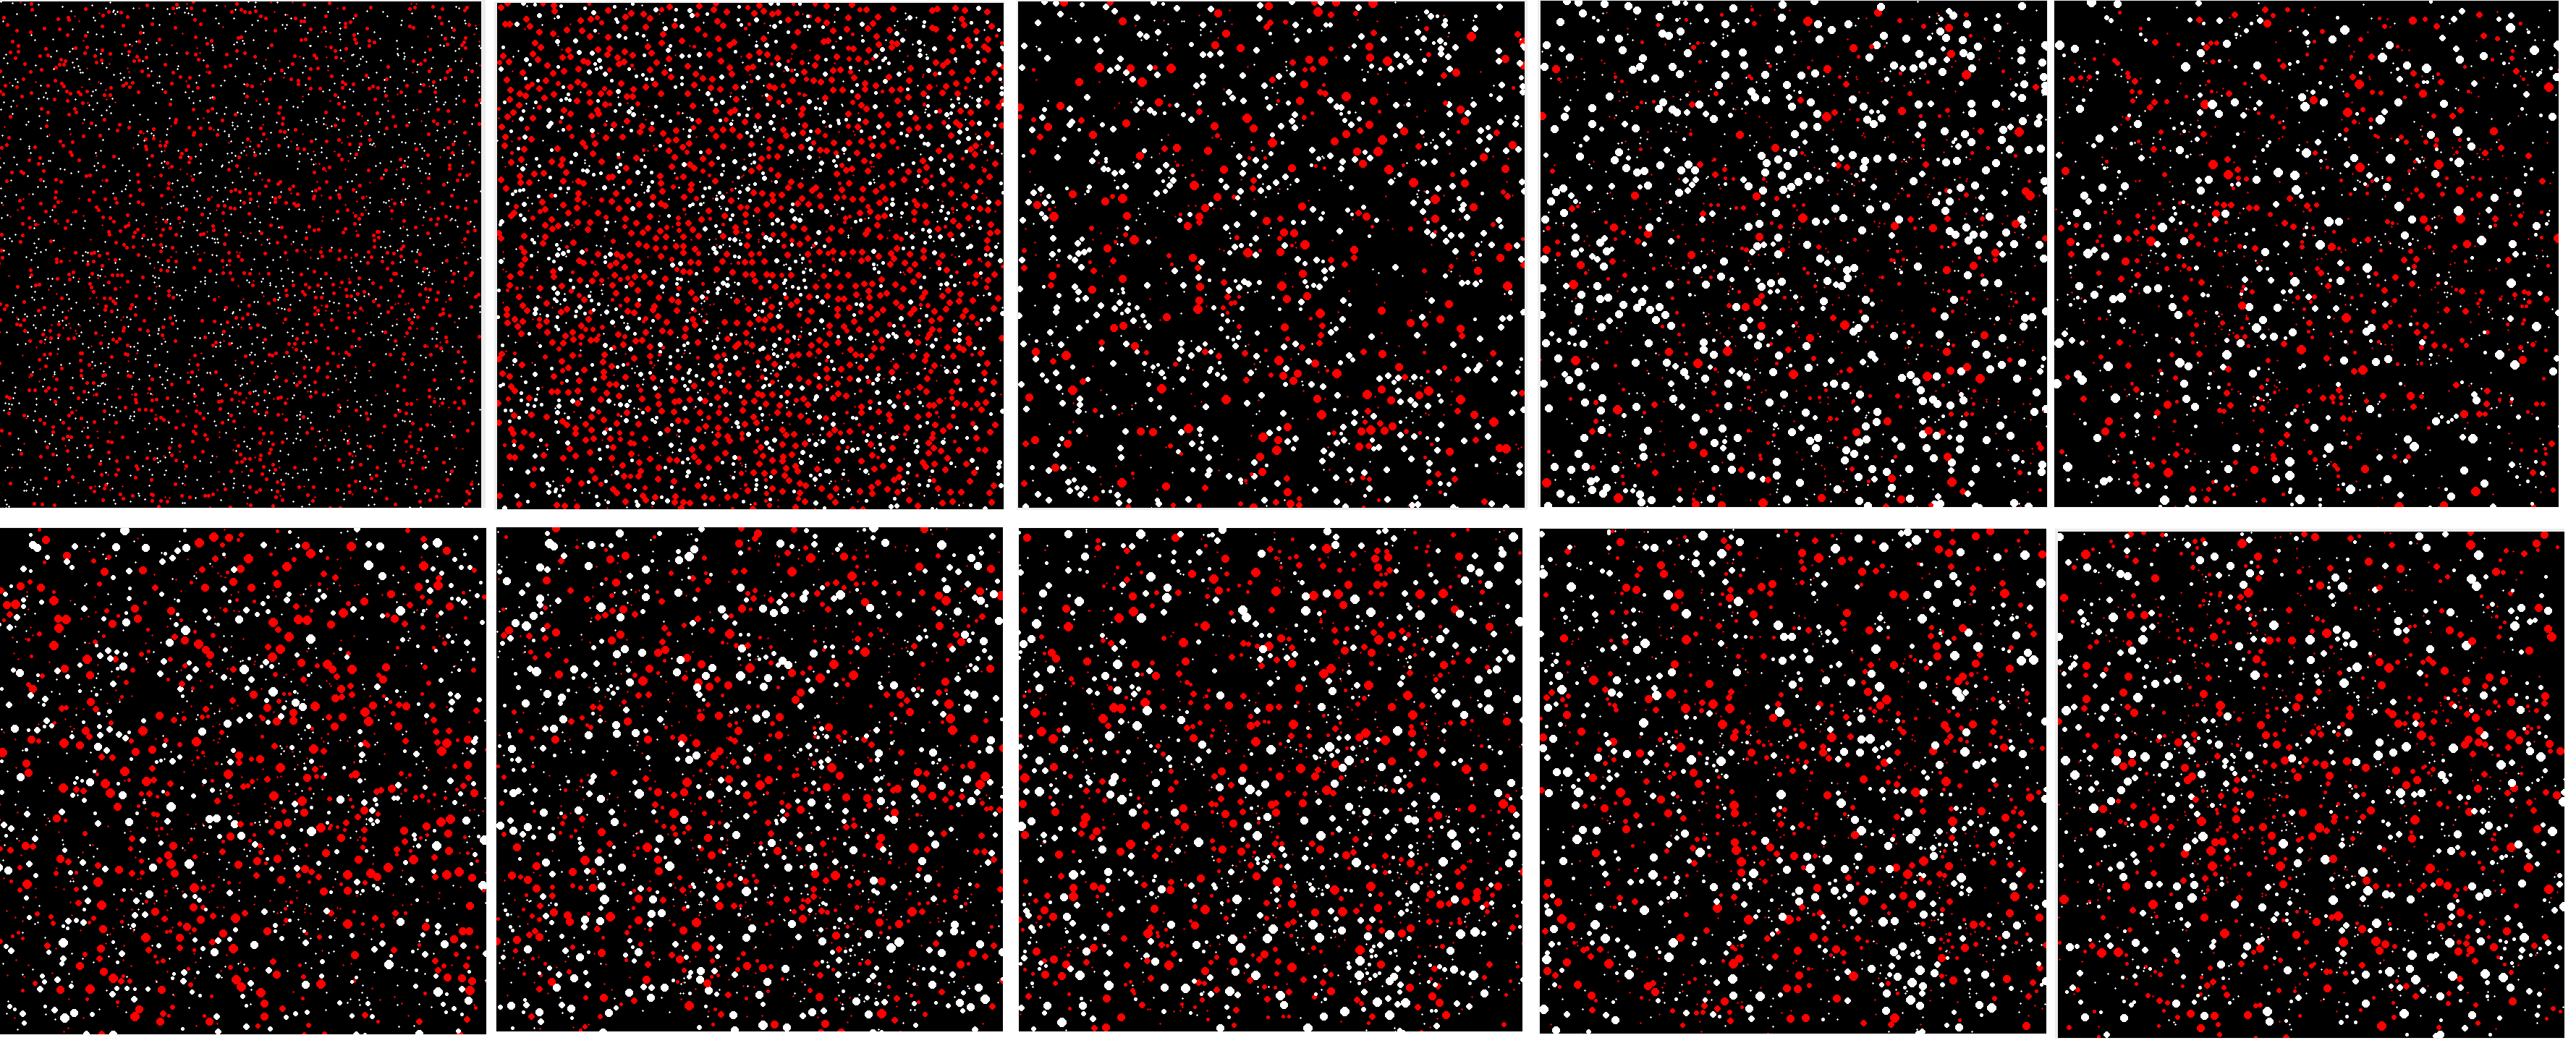
\includegraphics[width=\textwidth]{succession_plants_render.png}
	\caption{ Succession Test: Appearance of the slow growing S$_{slow}$ (white) and fast growing S$_{red}$ (blue) at different times during the simulation. From left-to-right, top-top-bottom: 10, 20, 30, 40, 50, 60, 70, 80, 90 and 100 years.}
	\label{fig:succession_plants_render}
\end{figure}

\textbf{PROPAGATION TEST}\\

The \textit{propagation} property simply states that plants \textit{propagate} in clusters surrounding the seed plants. To ensure propagation is modelled in the ecosystem simulator a simulation is run with a single starting grass seed (see appendix \ref{AppendixB} for specie details) and its evolution tracked throughout. Figure \ref{fig:propagation_test_render} shows that iterative propagation through annual seeding enables a single seed plant to colonize the entirety of the terrain. \\

\begin{figure}
\center
	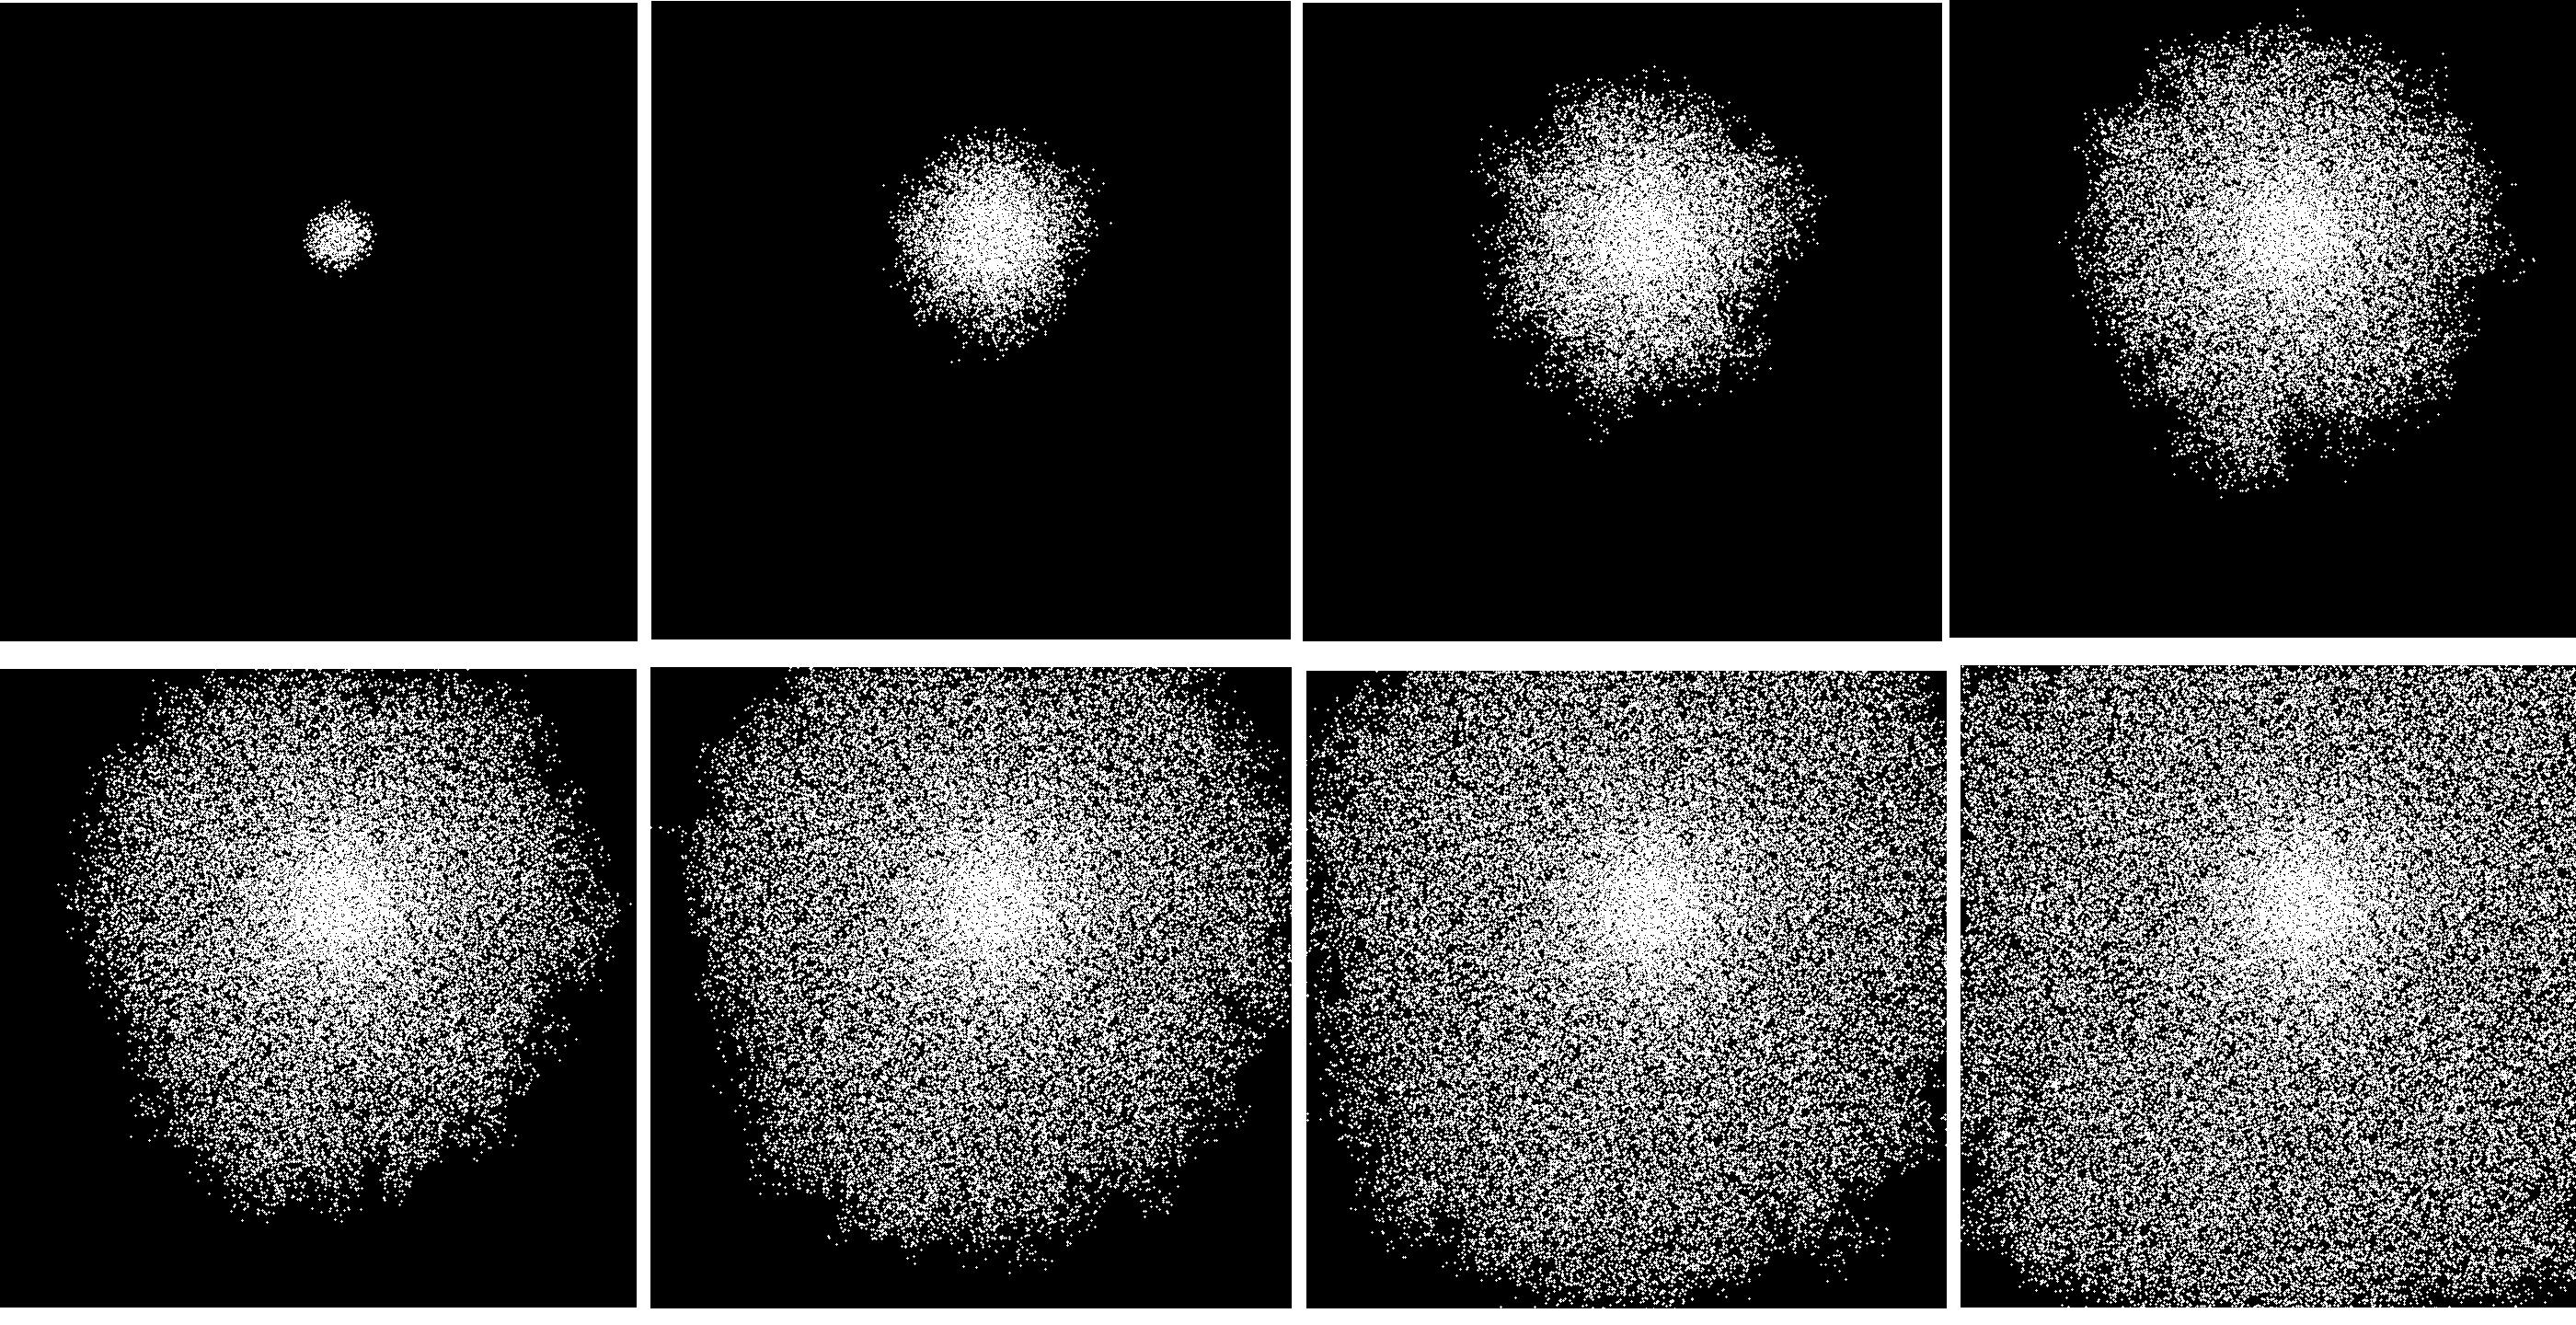
\includegraphics[width=\textwidth]{propagation_test_render.png}
	\caption{ Propagation Test: Evolution through time of a simulation starting from a single seed plant of grass. From left-to-right, top-to-bottom: 2, 10, 20, 30, 40, 50, 60, 70 years in.}
	\label{fig:propagation_test_render}
\end{figure}

\textbf{VARYING RESOURCE TEST} \\

To ensure a given plant specie thrives better when the environments is better suited, multiple simulations are run with only specie \textit{S$_{base}$} (see appendix \ref{AppendixB} for specie properties) varying only in available humidity (see table \ref{tab:varying_resource_test_simulations} for details on the resources of each simulation run). Throughout the simulation, the average plant canopy width is tracked to monitor the strength of the plants. As can be seen by the results plotted in figure \ref{fig:varying_resource_test}, plants strive better in environments better suited to their resource requirements.\\

\begin{table}[]
  \centering
	    \begin{tabular}{|p{2cm}|p{2cm}|p{2cm}|p{2cm}|p{2cm}|p{2cm}|}
		\hline
		\textbf{Simulation} & \textbf{Simulation time (years)} & \textbf{Humidity} & \textbf{Illumination} & \textbf{Temperature} & \textbf{Slope}\\
		\hline         
		1 & 100 & 22 & 10 & 20 & 0\\           
		\hline       
		2 & 100 & 24 & 10 & 20 & 0\\
		\hline       
		3 & 100 & 26 & 10 & 20 & 0\\           
		\hline     
		4 & 100 & 28 & 10 & 20 & 0\\           
		\hline     
		5 & 100 & 30 & 10 & 20 & 0\\           
		\hline       
		6 & 100 & 32 & 10 & 20 & 0\\           
		\hline       
		7 & 100 & 34 & 10 & 20 & 0\\           
		\hline      
		8 & 100 & 36 & 10 & 20 & 0\\           
		\hline       
		9 & 100 & 38 & 10 & 20 & 0\\           
		\hline     
		\end{tabular}
		\caption{Varying resource test: Resource configurations for each simulation run. For simplicity, monthly resources are kept constant.}
		\label{tab:varying_resource_test_simulations}
\end{table}

\begin{figure}
\center
	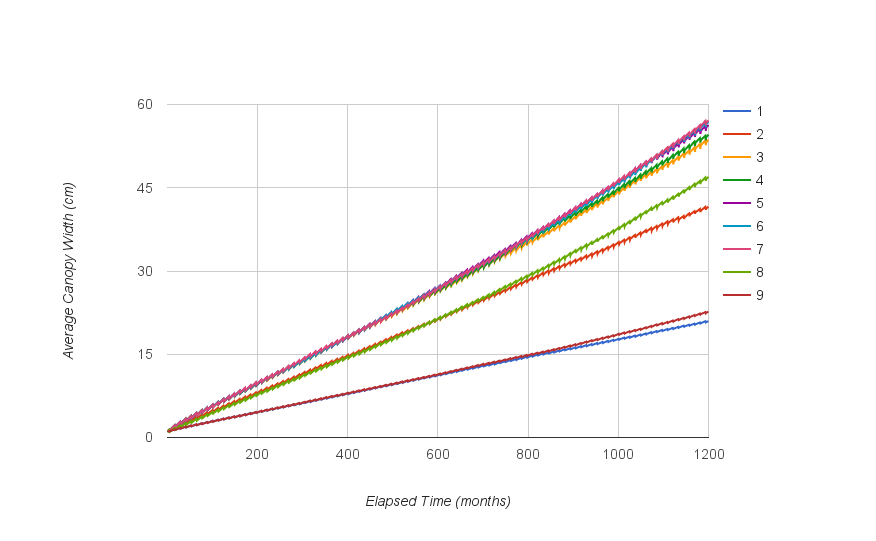
\includegraphics[width=\textwidth]{varying_resource_test.png}
	\caption{ Varying resource test: Average canopy width throughout the simulation with only plant specie \textit{S$_{base}$} and resources configured as outlined in table \ref{tab:varying_resource_test_simulations}. It shows that the average canopy width is low when the configured humidity is outside the species optimal humidity range (graphs 1 and 9), improves as it approaches optimal range (graphs 2 and 8) and reaches it's peak when the humidity is within the optimal range (graphs 3,4,5,6 and 7).}
	\label{fig:varying_resource_test}
\end{figure}

\textbf{SHADE TEST}\\

Plants that are heavily dependent on illumination struggle to grow in areas shaded by the canopy of larger plants. To ensure this is modelled in the ecosystem simulator, a simulation is run with two species: \textit{S$_{smallroots}$} and grass (see appendix \ref{AppendixB} for specie details). \textit{S$_{smallroots}$} is a custom specie created for the purpose of this test which has very small roots growth. This is important so as to focus on the effects of illumination and minimize the influence of drought. Figure \ref{fig:shade_test}, which illustrates the state of the simulation after fifty years, shows the grass struggling to grow in areas directly below the canopies of \textit{S$_{smallroots}$}.\\

\begin{figure}
\center
	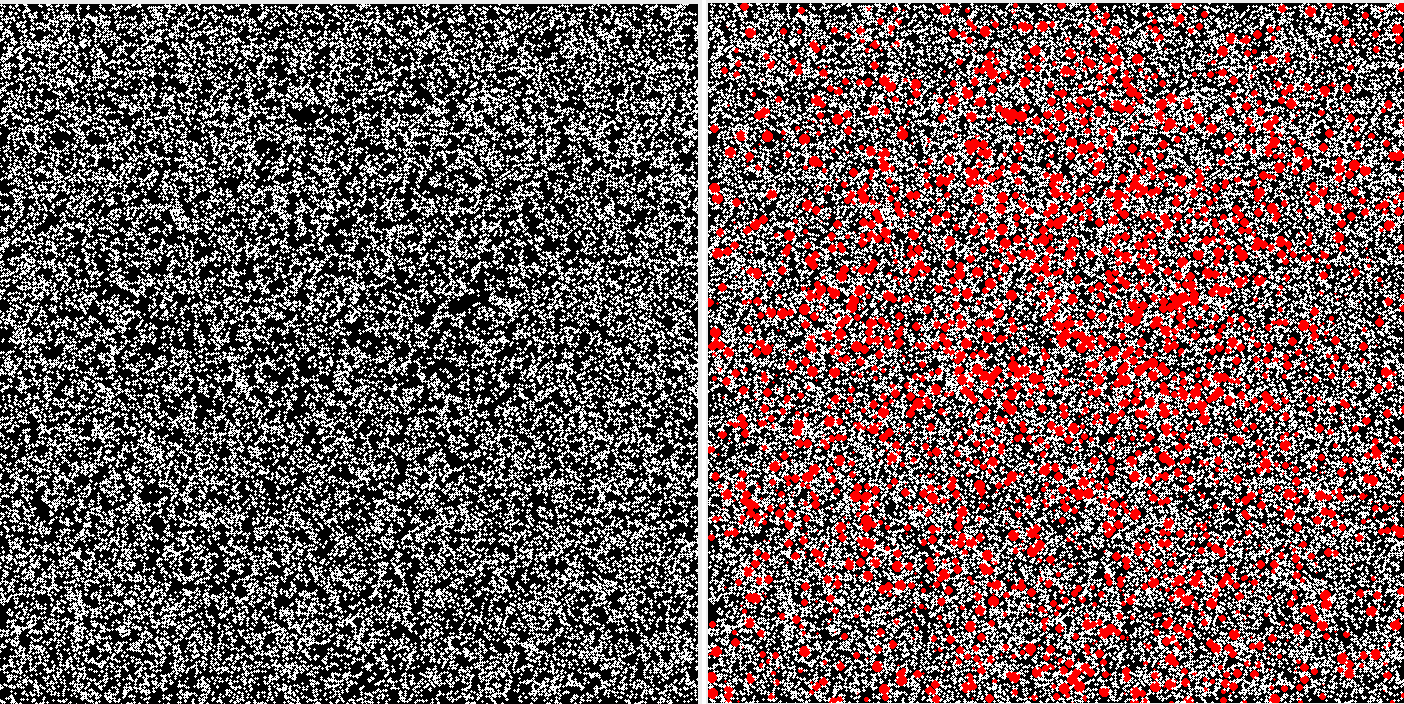
\includegraphics[width=\textwidth]{shade_propagation_test.png}
	\caption{ Shade Test: Results of a simulation run with \textit{S$_{smallroots}$} (red), grass (white) after fifty years. Rendered with \textit{S$_{smallroots}$} (right) and without (left) to clearly visualise the effects of shade.}
	\label{fig:shade_test}
\end{figure}

\textbf{SHADE-LOVING TEST}\\

As discussed in \ref{subsec:spawning_plants}, species which strive in shaded areas are deemed shade-loving. The shade can be caused by the terrain relief or by the shadow cast by the canopy of taller plants. To test whether the ecosystem simulator successfully caters for such plant species, a simulation is run identical to that done in the shade test but with shade-loving specie \textit{S$_{shadeloving}$} added (see appendix \ref{AppendixB} for specie details). As seen by the snapshot of the simulation after fifty years illustrated in figure \ref{fig:shade_loving_test}, instances of \textit{S$_{shadeloving}$} only appear in areas covered by the canopies of \textit{S$_{smallroots}$}.

\begin{figure}
\center
	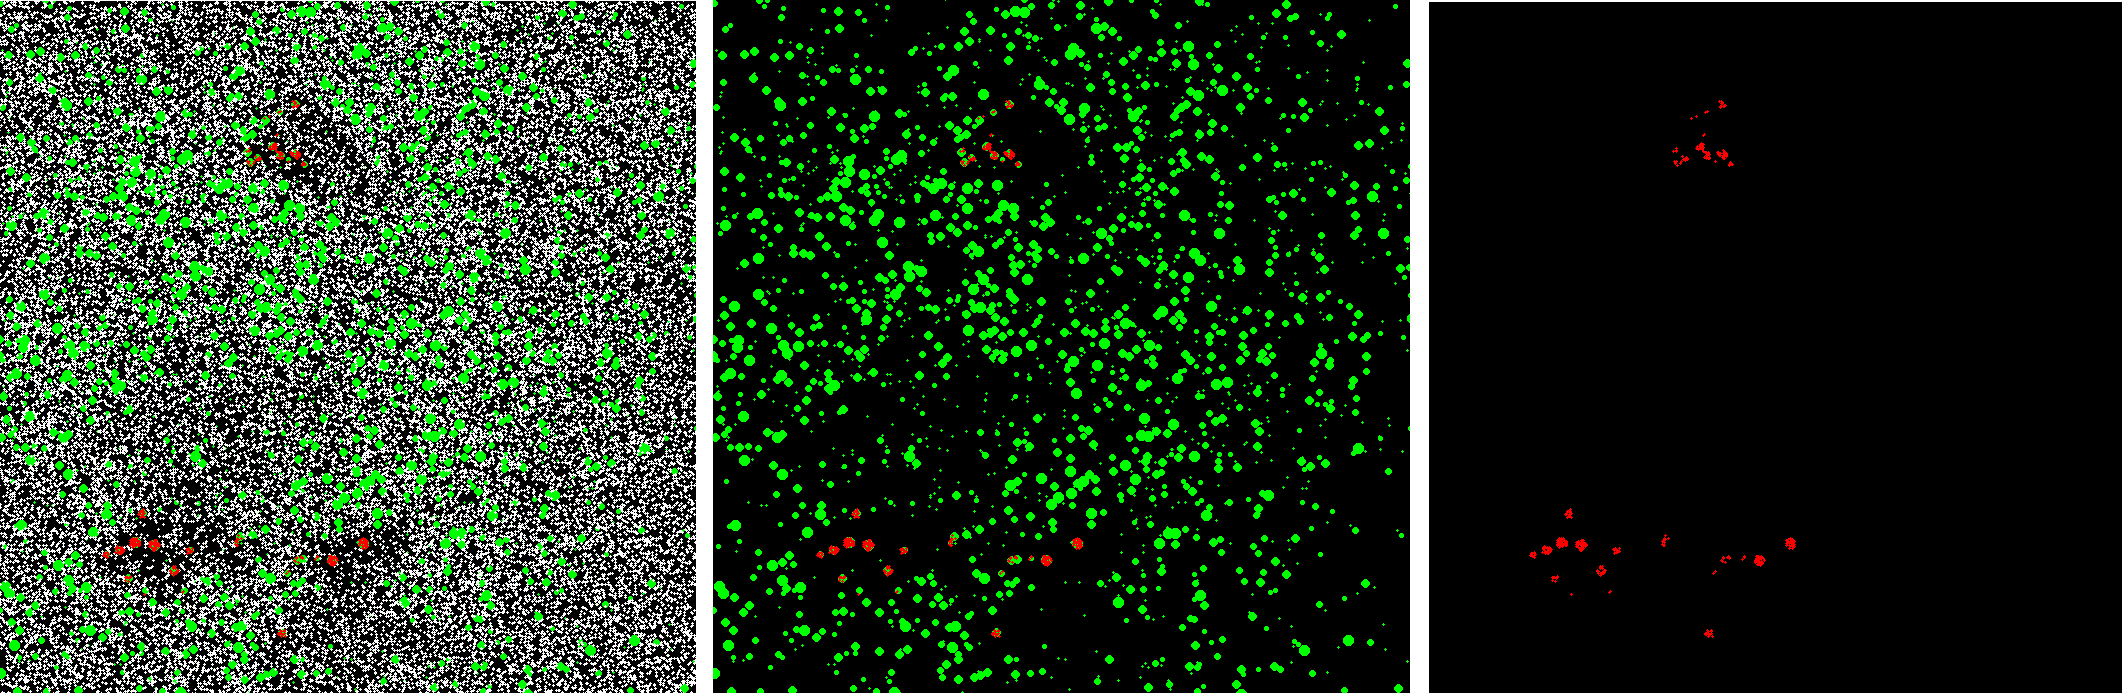
\includegraphics[width=\textwidth]{shade_loving_test.png}
	\caption{ Shade Loving Test: Simulation with \textit{S$_{smallroots}$} (green), grass (white) and \textit{S$_{shadeloving}$} after fifty years. From left-to-right: All species, excluding grass and only \textit{S$_{shadeloving}$}. As can be seen, \textit{S$_{shadeloving}$} strive under the canopies of \textit{S$_{smallroots}$}.}
	\label{fig:shade_loving_test}
\end{figure}
